\documentclass[]{article}

\usepackage{color}
\usepackage{graphicx}
\usepackage{amsmath}
\usepackage{amsfonts}
\usepackage{mathrsfs}
\usepackage[symbol]{footmisc}
\newcommand{\red}[1]{\textbf{\color{red} #1}}

\newcommand{\revision}[1]{\textbf{#1}}
\usepackage[margin=1.5in]{geometry}

\setlength{\parindent}{0pt}
\setlength{\parskip}{0.5\baselineskip}

%opening
\title{Response to Reviewer 1}
\author{}
\date{}

\begin{document}

\maketitle

We are pleased with the positive assessment of our work by the reviewer and thank him/her for thoroughly reading our manuscript and for providing constructive input. The reviewer justly gives suggestions for interesting additional optimal control cases. Although computational costs prohibit us from running these cases in an acceptable timeframe during the revision process, they are subject of current research and will be included in future work. The responses to the reviewer's comments and adaptations in the revised manuscript are discussed below.

\hrulefill

\paragraph{Reviewer} \textit{The present article investigates the improvement on wind-farm power by performing different wind turbine optimization strategies (yaw and induction) modeled using large-eddy simulations (LESs) combined with an adjoint-based optimization method. Two test cases are considered, one characterized by uniform incoming flow conditions (turbulence void), and another where a precursor LES is used to seed inflow turbulence in the domain containing the 4 x 4 wind turbines layout. The authors present new results about combining axial induction and dynamic yaw control. Although for the relatively small wind farm under consideration, the yaw control over-performs induction control, the authors present interesting analysis on the potential of combining the two methods. The manuscript is overall well written and organized, and the majority of the results are correctly interpreted and clearly articulated. Therefore, I recommend publication after minor 	revisions are made. Here below a list a series of concerns/clarifications that need to be addressed prior to its publication.}


\section*{Comments}
\hrulefill

\paragraph{1. Reviewer} \textit{The authors use an actuator disk model that does not account for rotational effects (line 158). However, in lines 362-364 the authors state that their LES model output exhibits curling of the wakes as a result of the control strategy. What is the impact of the nonrotating actuator disk approach on wake curling and turbine control? It would be interesting to repeat on of the cases, in particular I3Y, including the tangential forces on the turbine, and report on the differences in the dynamics as well as power extraction and wind farm efficiency found.}

\paragraph{Response} We thank the reviewer for this comment. Indeed, a non-rotating actuator disk model (ADM) is used in the current study. In a recent paper by Howland \emph{et al.} [24], the wake structure behind turbines in yaw was studied using both experimental and numerical techniques. It was found that both a non-rotating ADM and a rotating actuator line model (ALM) produce similar curled wakes, and that the wake center was deflected to a similar degree in both models. The main dissimilarity in the wakes from both models is a rotation-induced top-down asymmetry in the ALM case. Therefore, it is expected that an ADM with tangential forces would yield similar results: a comparable wake deflection with rotation-induced top-down asymmetry. Therefore, the prevailing control mechanisms identified in the current paper are expected to also be found in more detailed turbine models, albeit with slight differences in e.g. yaw angles of the upstream turbines.

We agree that performing optimal yaw control simulations with more detailed turbine models would yield interesting results for comparison with the current ADM. This is subject of parallel ongoing work. 

We have included the explanation above in the revised manuscript as follows:
\begin{itemize}
	\item Section 4.2.2 (Static yaw regime - wake redirection, \red{line XX, p YY}): \\``... redirecting the wakes sufficiently. \revision{It is important to note that such wake redirection and curling is not simply an artifact of the currently used non-rotating ADM, since similar wake characteristics were also observed in rotating actuator line models [24].} The static yaw wake ...''
	\item Section 5 (Conclusions and future work, \red{line XX, p YY}): \\``\revision{The current optimization studies have been performed using relatively simple non-rotating actuator disk models for the wind turbine rotors without the inclusion of towers or nacelles. Although it has been shown that, by using this approach, the fidelity of far wake characteristics is satisfactory, the credibility of the current power gains and control strategies in practice could be further increased through wind-tunnel testing and similar optimization studies with more detailed turbine models, e.g. by adding drag forces for the tower and nacelle or by representing the rotor with an actuator line model. These are left for future work.} Finally, note that the current study optimizes power at all costs, and did not account for any undesirable loading characteristics. These should also be considered upon thoroughly comparing induction and yaw control for practical purposes. \revision{In this latter case, a detailed turbine representation is of high importance.}''
\end{itemize}

[24] M. F. Howland, J. Bossuyt, L. A. Martinez-Tossas, J. Meyers, C. Meneveau, ``Wake Structure of Wind Turbines in Yaw under Uniform Inflow Conditions'' Journal of Renewable and Sustainable Energy 8, 043301 (2016)

\hrulefill 

\paragraph{2. Reviewer} \textit{Figure 12a displays a strong power recovery for rows 3 and 4 for the cases where yaw control is applied (this effect is less evident for the induction control cases), which results in a wind farm efficiency increase of ~20\% with respect to the reference case. I wonder how much of that improvement is due to the reduced number of wind turbine rows (only 4), and the ability to quickly adjust to a much higher power extraction level as the end of the wind farm is approached. It would be desirable to perform at least one more simulation (I3Y) with an extended domain and wind farm, doubling the number of turbine rows from 4 to 8. Such case will reveal the trend of the increase in power extraction and wind farm efficiency as the size of the wind farm is enlarged, and will help extrapolate to what the gain would be for a more realistic wind farm size. In addition, the authors could consider another case where the use of periodic boundary conditions in the streamwise direction, as an asymptotic limit for an “infinite” wind farm, allowing to keep the size of the simulation (although not informative of row dependency within the wind farm). These two additional cases will further increase the robustness of the analysis and conclusions regarding the combined induction/yaw control approach proposed, and the finite wind farm effects.}

\paragraph{Response} This is an important comment. We agree that the current layout is very suited for wake redirection through yaw control. More specifically, the relatively short streamwise extent of the farm and the aligned layout are favorable for wake redirection since wakes do not interact with downstream turbines in other columns. 

The desired additional I3Y case suggested by the reviewer is subject of current research and has been submitted in a conference paper at the Science of Making Torque conference in June. In this work, we will perform induction, yaw, and combined control (equivalent to I3, Y, and I3Y) for wind farms with 12 turbine rows in both aligned and staggered conditions such that we can draw properly funded conclusions for larger wind farms with various layouts. The computational time of these simulations however disallow them to be included in the current paper. 

In the submitted version of the manuscript, we already indicated in the summary that the quantified relative profitability of induction versus yaw control have to be interpreted with the given wind-farm layout in mind. 

In the revised version of the manuscript, we have made this remark more explicit by mentioning this every time the power gains of yaw control are compared to induction control, i.e.: 
\begin{itemize}
	 \item Abstract (\red{line XX, p 1}): \\ ``... We study a 4 $\times$ 4 aligned wind farm, and find that \revision{for this farm layout} yaw control is more effective than induction control. ...''
	 \item Section 4.2.1 (Uniform inflow power extraction, \red{line XX, p YY}): \\``... close to freestream conditions. \revision{Remark that the favorability of yaw over induction control is quantified here for a relatively small set of aligned, and care should be taken when extrapolating these results to wind farms of larger size and/or different layouts (see further discussion in Section 5).}''
	 \item Section 4.4 (Discussion, \red{line XX, p YY}): \\``... for the current setup \revision{with a relatively small aligned wind farm}, all yaw-enabled cases consistently outperform cases based solely on axial induction control. ...''
	 \item Section 5 (Conclusions and future work, \red{line XX, p YY}): \\``...depending on their position within the farm. \revision{Moreover, also the wind-farm layout is expected to affect which control mechanism yields more power gains, e.g. the opportunities for wake redirection in aligned wind farms are much better than in staggered wind farms, where deflected wakes will more easily hit turbines in neighboring columns. The question of which control strategy is more effective in larger wind farms with various layouts is subject of current investigation.} ''
\end{itemize}



The suggested infinite wind farm optimal control case as suggested by the reviewer has been performed for induction control in Goit \& Meyers 2015, J Fluid Mech 768. Comparing optimal control in periodic farms to finite farms can be problematic: experience has shown that the optimizer tends to increase power by slowing down the overall boundary layer in a transient manner and in infinite farms, requiring an ad-hoc penalty term to be used by Goit \& Meyers. This large-scale slow-down is not possible in finite wind-farms, where the inlet is prescribed by the precursor simulation. \red{The entire idea of using power gains from infinite farms to draw conclusions for finite farms is hence questionable, and warrants its own further investigation which is out of scope of the current work.} 

\hrulefill

\paragraph{3. Reviewer} \textit{Line 226-230. How is that time related to an eddy and advection scales? What are the implications going to real large-scale forcing variability? Please comment on that.}

\paragraph{Response} Regarding the relation of the user-defined time horizons we have related them to the characteristic timescale of the wind farm, i.e. the wind-farm flowthrough time as follows (\red{line XX, p YY}):

``
... total control time of 900~s.  \revision{Note that, given a wind-farm length of $3 \times 6D = 1 800$ m and a free-stream velocity $U_\infty = 8$ m s$^{-1}$, the wind-farm flowthrough time is approximately 225 s. Hence, the total control time comprises about 4 flowthroughs, and the optimization horizon within each window covers about 1.33 flowthrough times. Because of the latter, each turbine row has the opportunity to take into account interaction with every downstream row, and the sensitivity of power gains to the optimization horizon $T$ is expected to be limited.} All time-averaged results ...
''

Regarding the implications of real large-scale forcing variability, the same time horizons could be used in principle. However, quantifying potential power gains for the different in an actual wind-farm site would obviously require to take annual variability in wind speed and direction into account. We added a comment on this in the Summary section (\red{line XX, p YY}): 

`` 
... atmospheric conditions for particular wind farms. \revision{Also, throughout this work we considered a constant wind direction and flow forcing. When quantifying potential power gains for real wind farms, the annual distribution of wind speed and velocities at the given site should be taken into account in the flow forcing.} ...
''

\red{Weet niet of eddy time scales hier echt relevant zijn...}

\hrulefill

\paragraph{4. Reviewer} \textit{Line 291-292. It would be beneficial to include the turbulent case also, making it a 4-panel figure. That case is more representative of an ABL flow and therefore provides the reader a better sense of the optimization convergence in a more realistic scenario.}

\paragraph{Response} As indicated in the text, the turbulent inflow case follows a similar behavior as the uniform inflow. Including both uniform and turbulent convergence characteristics would in our opinion draw the attention away from the more important results in the paper. As a compromise, we replaced the uniform optimization convergence with the turbulent one in the revised manuscript (also shown below).

\begin{figure}[h]
	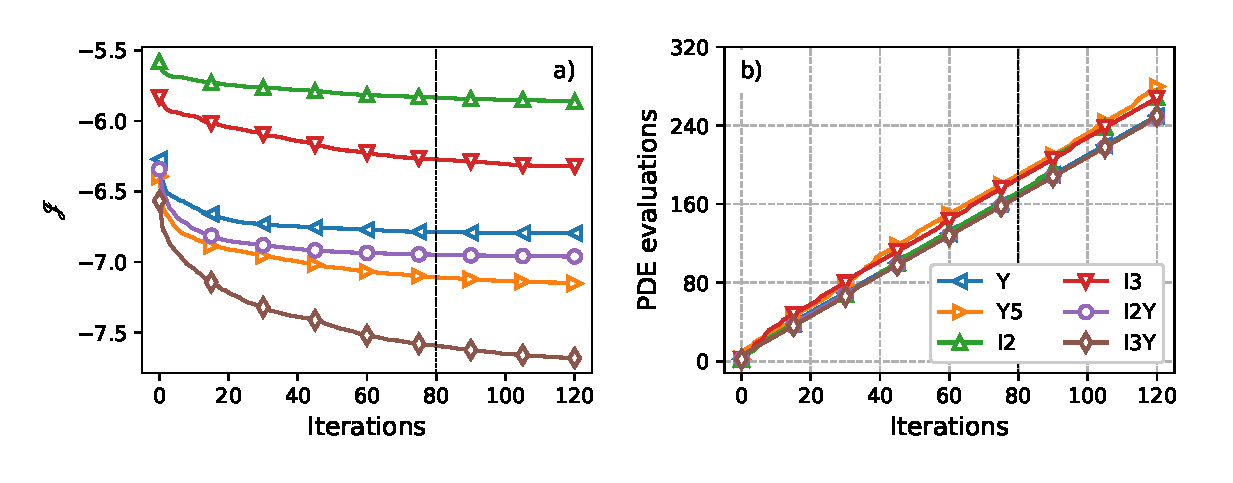
\includegraphics[width=\textwidth]{figure4_revised}
	\caption{Convergence behavior for the second optimization window in \revision{turbulent} inflow. \emph{a) }: Cost functional $\mathscr{J}$. \emph{b) }: PDE evaluations (forward or adjoint). Markers represent every fifteenth iteration step.}
\end{figure} 

\hrulefill

\paragraph{5. Reviewer} \textit{Line 382-385. What about the peak that shows up in all case for $St < 0.1$ ($\approx$ 0.05)? Please explain.}

\paragraph{Response} This peak, occuring at the first non-zero frequency, is an artifact of the way the spectral density estimates are computed. The data is detrended by removing the mean before computing the PSD estimate using Welch's method, which divides the data in overlapping windows for increased statistical convergence. This can cause loss of frequency resolution in the lowest frequencies of the spectrum resulting in energy bleeding into other frequencies including the zero frequency which represents the mean component (which should be zero in theory due to the removal of the mean). We fixed this by simply not detrending the data prior to computing the PSD estimate, resulting in a smooth behavior at the lowest frequencies with no spuriously apparent peaks. 

The large spectral content at low frequencies points towards long-time trends in the yaw angles, e.g. for turbines transitioning from the meandering regime $(\overline{\theta} = 0^{\circ})$ to the redirection regime $(\overline{\theta} = 30^{\circ})$. The revised versions of figures 9 and 15 are shown below. \red{WM: Denk niet dat we hier expliciet in de tekst naar moeten verwijzen? Lijkt me vrij self-explanatory..}

\begin{figure}
	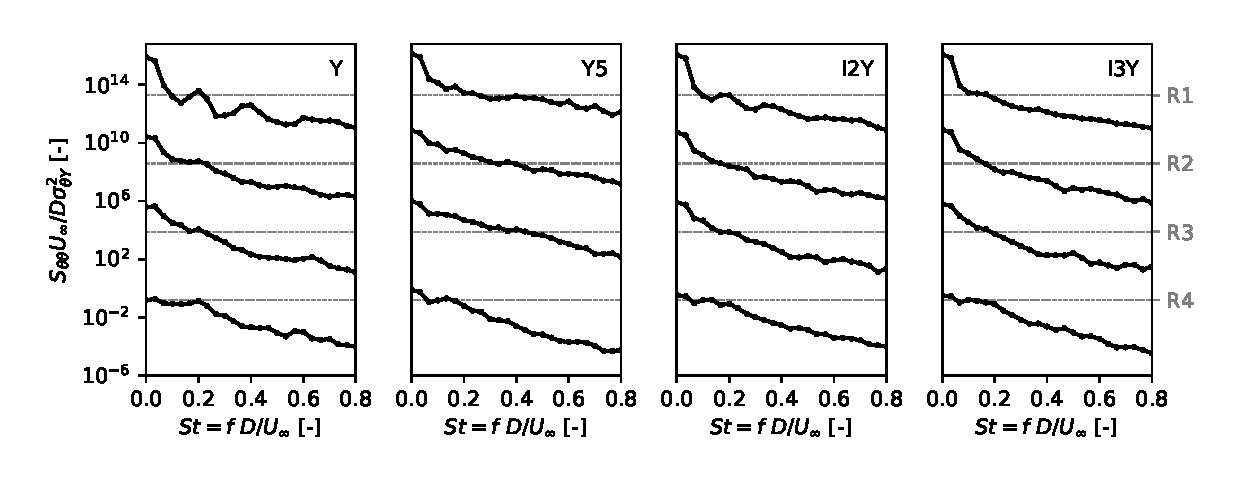
\includegraphics[width=\textwidth]{figure9_revised}
	\caption{Revised version of Figure 9. See revised manuscript.}
\end{figure}

\begin{figure}
	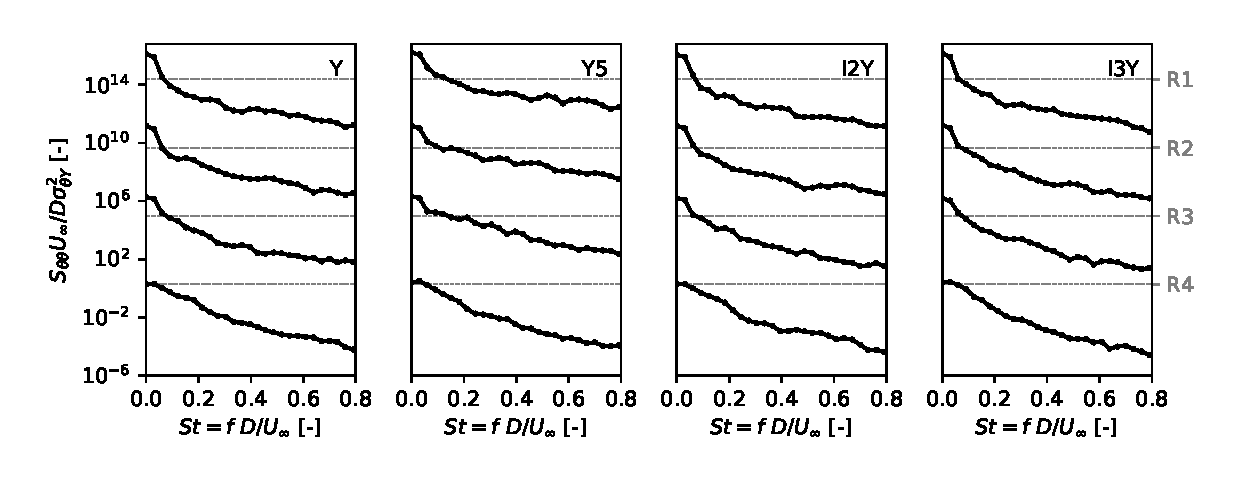
\includegraphics[width=\textwidth]{figure15_revised}
	\caption{Revised version of Figure 15. See revised manuscript.}
\end{figure}

\end{document}
